\section{Approach}

\subsection{Gaze Tracking}

For our gaze tracking component, we investigated a few different approaches to gaze tracking as documented in the survey of gaze tracking performed by Chennamma and Yuan~\cite{chennamma2013survey}. As depicted in the survey, the most accurate ways to track gaze is with special hardware, which is typically of the form 

\begin{enumerate}
    \item A wearable headset that has two cameras pointed into the eyes, this provides a very accurate gaze that can be approximated by a gaze vector which can then be correlated to a approximate region with a margin of error. This approach is the most effective, and allows the user to move their heads around and still be effective. 
    \item Multiple infrared cameras that are mounted at two different locations that use the infrared light to illuminate the pupils. This provides an accurate approach as well, and allows for head movement within a certain range. 
    \item A single camera can be used to detect pupils (eye tracking); however they can't reliably detect a vector where the eyes are looking. A single camera also does not allow a user to move their head.
\end{enumerate}

Since we are using limited equipment for the ASS suite, we decided to use option (3) and tweak an existing library to derive a form of gaze. We used an reference implementation of Fabian Timm's algorithm~\cite{EyeTrackingTIMM} which is capable of deriving bounding boxes. 

Our eye tracking pipeline functions as follows:

\begin{enumerate}
    \item Using OpenCV's \href{https://docs.opencv.org/3.4/db/d28/tutorial_cascade_classifier.html}{cascade classifier}, we attempt to detect the available faces in the image. For this we are using a pre-trained cascade file that is designed for frontal facing images.
    \item If no face is detected, do nothing. Otherwise, we can attempt to find the eyes.
    \item Divide the found face into two regions, each region will contain one eye as the face is a fairly centered bounding box. We can derive a relative eye region by partitioning the face with some constant values.
    \item Using the eyeLike library~\cite{trishume} (reference implementation of Timm's algorithm), find the center of the eye (pupil).
    \item Derive and draw rectangle based on the previously found bounding boxes, place the pupil inside the rectangle. 
    \item At this we know where the pupil is relative to a bounding box; however, we have not estimated gaze. Thus, we normalize all the values of the eye region and eye center to be relative to the bounding boxes 
    \item We then consider a one-dimensional plane (a line in the x-axis) which starts at the minimum edge of our bounding box, ends at the maximum edge of the bounding box, and then uses the pupil position as the point on the line. See diagram below
    \begin{center}
        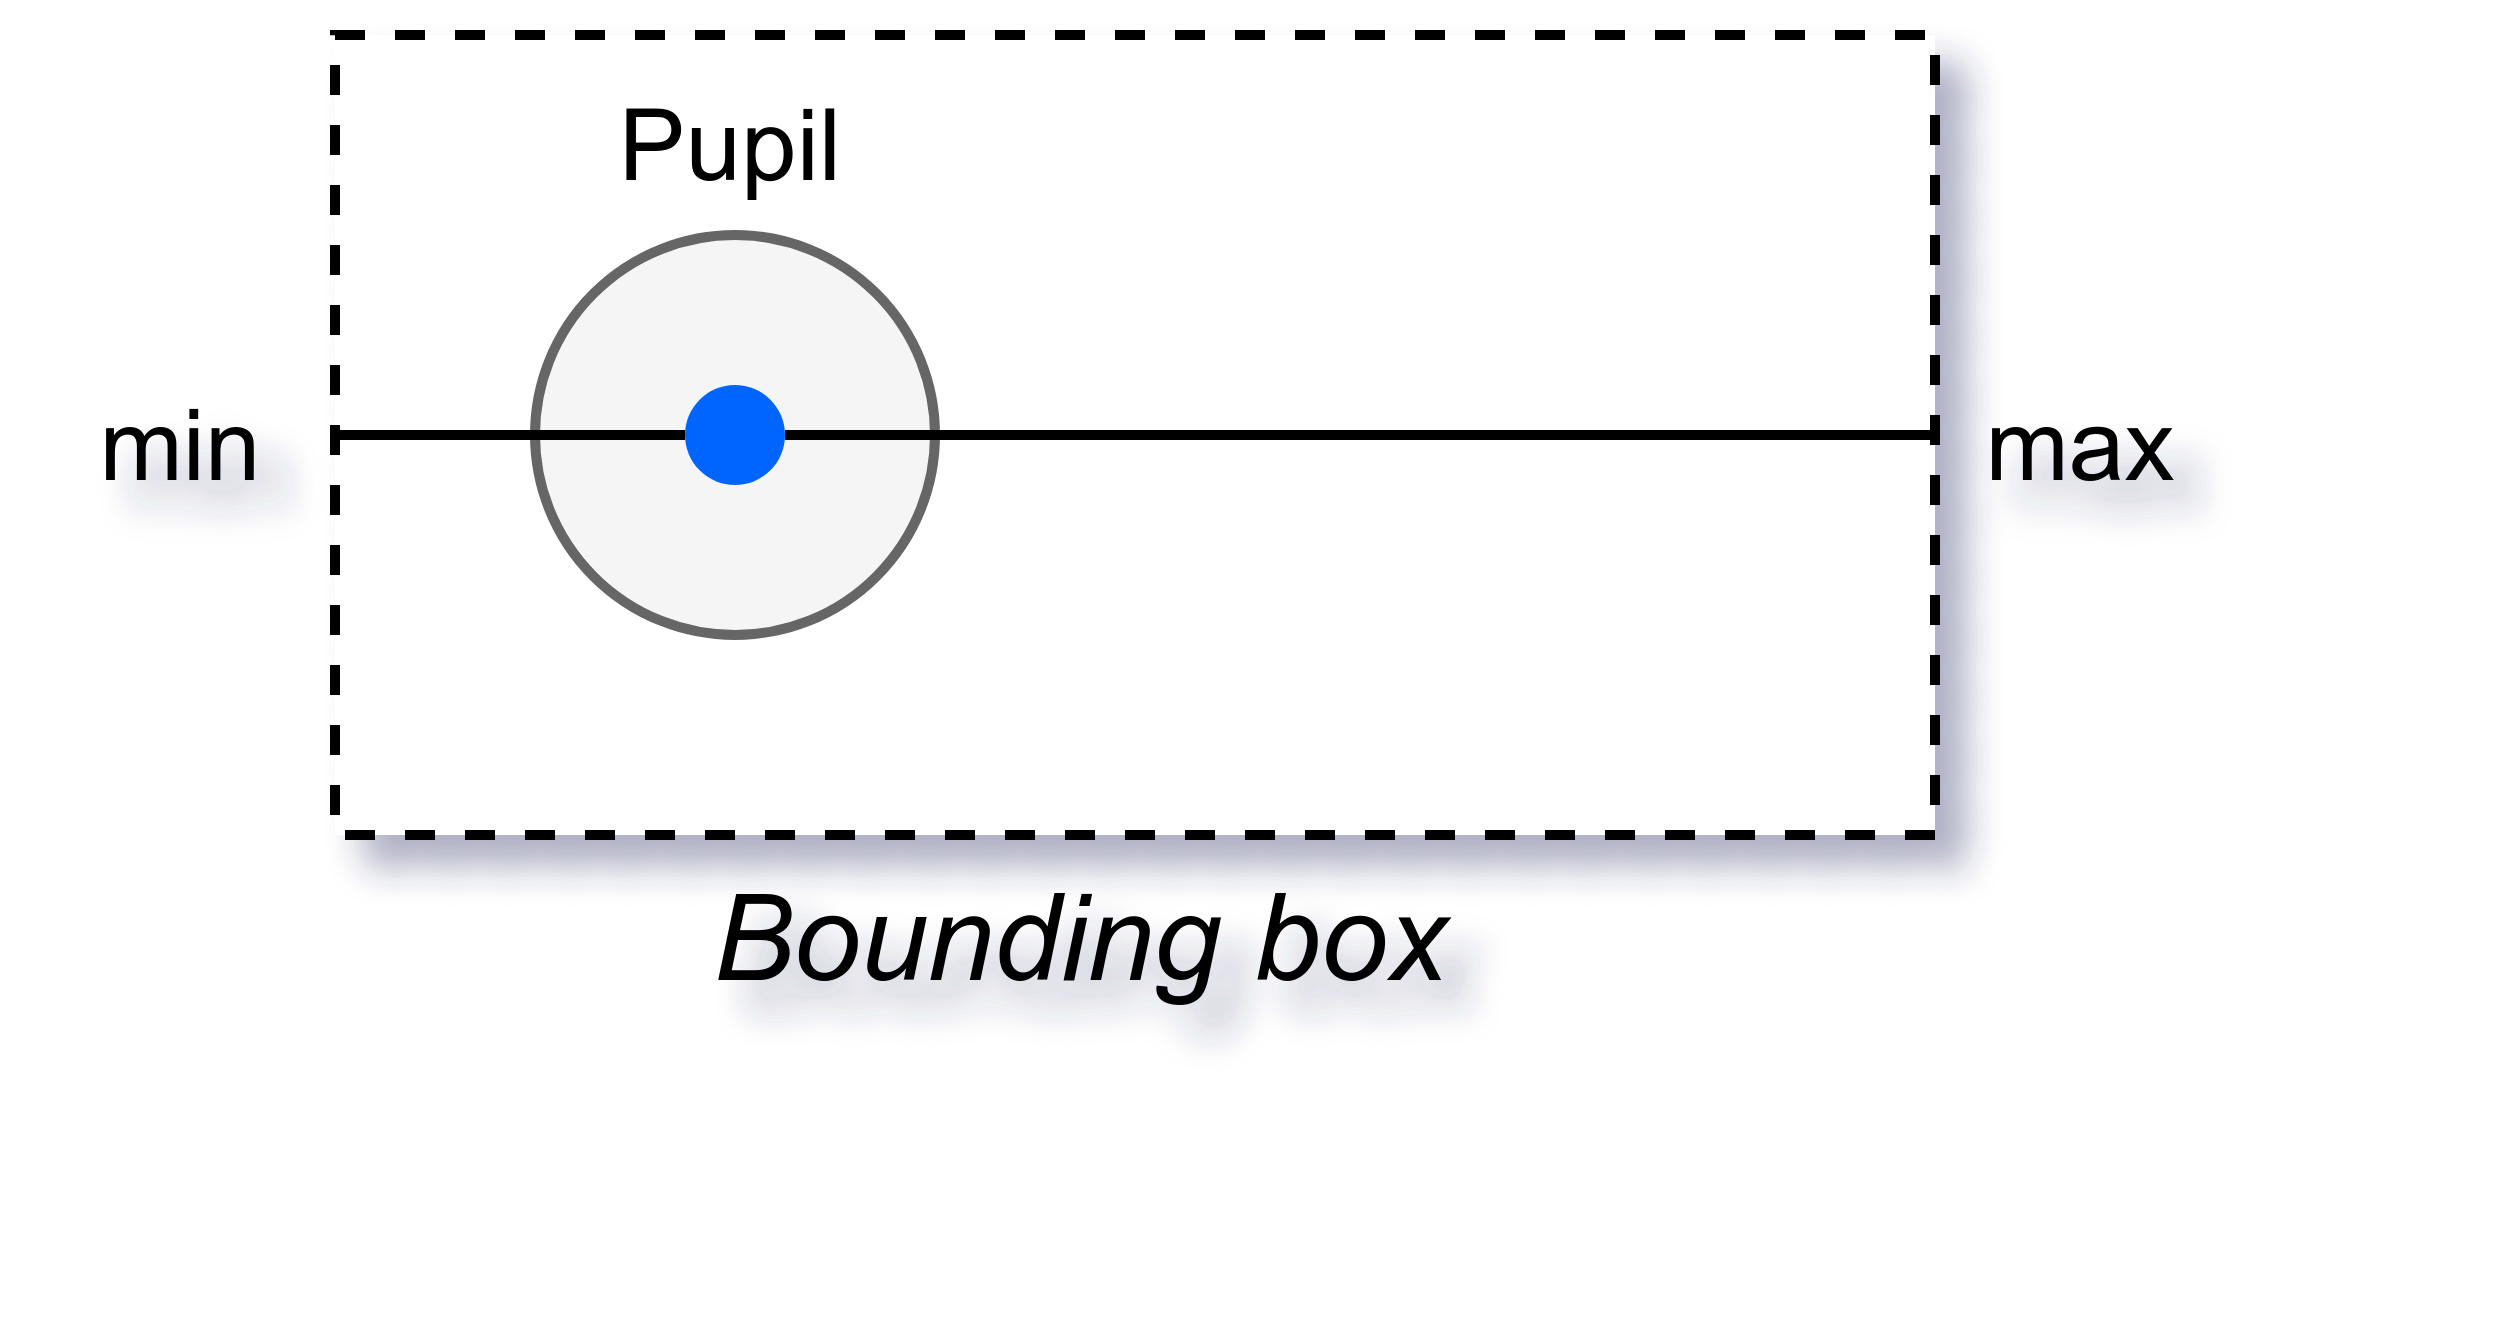
\includegraphics[width=0.5\linewidth]{figures/EyeLoc.png}
    \end{center}
    Between the min and max values is the pupils location, this can be used to derive a percentage as follows (assuming the coordinates have been normalized to min):
    \[
        \frac{pupil.x}{max.x}
        \]
    This percentage is the percentage to the left or right, where 50\% is dead center.

    \item We average the percentages between left and right eyes to derive an overall percentage.
    \item After some testing, we determined if the eye location is less than 40\% the eye is pointed right, if the eye is more than 60\% the eye is left, else the eye is centered.
    \item We render the findings to the mat, update our application's centralized eyeState value, and return.
\end{enumerate}


\subsection{Pedestrian Tracking}
Pedestrian tracking is achieved through a single function which takes in a \emph{cv::Mat} object that represents the current frame of the video and returns a custom data structure called \emph{PedTrackingResult}. The function initializes an instance of OpenCV's \emph{HOGDescriptor} object. With the help of OpenCV, this object can be passed a human detection method which can be passed to the \emph{HOGDescriptor}. Once this method is passed to the \emph{HOGDescriptor}, a clone of the original frame is produced. From here, the process of identifying humans in the frame is done by the work of the \emph{HOGDescriptor} using its \emph{detectMultiScale()} function after converting the input frame from four channels to one channel as needed by the function. This function produces a vector of \emph{cv::Rect} objects representing the bounding boxes for human-shaped objects in the frame and the weights associated with these bounding boxes. From here each \emph{cv::Rect} object in the frame is drawn onto the frame with its associated weight. The resulting frame and \emph{cv::Rect} vector is returned to the image pipeline in order to display the frame and to calculate driver attentiveness.\\

With the returned vector we first calculate the centre of the width for each \emph{cv::Rect} object. We then compare this center pixel against which third of the main video width the bounding box's centre lies in. We then compare the current eye state to this pedestrian object state and see if the driver is looking at the same third. This process is applied to each bounding box until the end of the list has been reached. Since there are three thirds of the window, if there are an even number of objects detected in each window then we can say that the minimum rate for attentiveness is a third of the total detected pedestrians. This means that if a driver pays attention to third with the most number of pedestrians then the minimum threshold needed for the classification to be passable for driving is $\frac{1}{3}$.

\subsection{Road Sign Tracking}

